%% Group 9, Big Data Analysis final report, in the ACM large two-column
%% format (acmart, acmtog) used by the course template.
%% Compile with XeLaTeX (author names contain Vietnamese characters):
%%   xelatex main; bibtex main; xelatex main; xelatex main
%% Numbers, tables, and figures are generated from the Kaggle outputs by
%%   HMDA_STYLE=acm python3 build_report_assets.py <results folder> <this folder>
%% The option nonacm removes the ACM rights block, journal footer, and
%% reference-format box, because this report is not an ACM publication.
\documentclass[acmtog,nonacm]{acmart}

\AtBeginDocument{%
  \providecommand\BibTeX{{%
    Bib\TeX}}}

\citestyle{acmauthoryear}

% The author names contain Vietnamese letters that pdfLaTeX cannot set in the
% ACM fonts, so stop early with a clear message if the wrong engine is chosen.
\ifPDFTeX
  \PackageError{main}{Compile this file with XeLaTeX (Overleaf: Menu, Compiler, XeLaTeX)}{The author names need XeLaTeX.}
\fi

\usepackage{tabularx}
\usepackage{enumitem}
\usepackage{xurl}
\newcommand{\fd}{\path}
\newcolumntype{L}{>{\raggedright\arraybackslash}X}
% generated by build_report_assets.py from the Kaggle run outputs; do not edit by hand
\newcommand{\nAll}{12,259,199}
\newcommand{\nApps}{10,781,992}
\newcommand{\nFirstLien}{7,981,147}
\newcommand{\nClosedEnd}{7,258,042}
\newcommand{\nNonBusiness}{6,694,328}
\newcommand{\nNonReverse}{6,690,389}
\newcommand{\nSiteBuilt}{6,088,849}
\newcommand{\nCore}{5,775,325}
\newcommand{\nOpenEndExempt}{216,601}
\newcommand{\nDecisioned}{4,514,505}
\newcommand{\nUsable}{4,100,051}
\newcommand{\nPricing}{3,616,549}
\newcommand{\nPricingUsable}{3,367,479}
\newcommand{\shareUsable}{90.8}
\newcommand{\nNonPrincipal}{313,524}
\newcommand{\shareNonPrincipal}{5.1}
\newcommand{\nDup}{26,755}
\newcommand{\nOriginated}{6,197,085}
\newcommand{\nPurchased}{1,276,504}
\newcommand{\nPreapproval}{200,703}
\newcommand{\rawDenialAll}{24.3}
\newcommand{\dbMatch}{all eight}
\newcommand{\drCore}{15.4}
\newcommand{\drConv}{13.2}
\newcommand{\drFHA}{21.8}
\newcommand{\drVA}{15.2}
\newcommand{\drUSDA}{12.1}
\newcommand{\drPurchase}{8.8}
\newcommand{\drRefi}{19.8}
\newcommand{\drCashout}{35.2}
\newcommand{\drHomeImp}{43.9}
\newcommand{\drOtherPurpose}{43.5}
\newcommand{\drFHACashout}{42.5}
\newcommand{\drConvCashout}{29.0}
\newcommand{\drFHAPurchase}{12.5}
\newcommand{\drConvPurchase}{7.6}
\newcommand{\nUSDAdec}{37,386}
\newcommand{\drDTIlowTwenty}{16.6}
\newcommand{\drDTItwentyThirty}{9.7}
\newcommand{\drDTIthirtyThirtysix}{8.8}
\newcommand{\drDTIfiftySixty}{24.9}
\newcommand{\drDTIoverSixty}{87.1}
\newcommand{\drDTImidMin}{8.5}
\newcommand{\drDTImidMax}{10.1}
\newcommand{\jumpConvMain}{+65.1}
\newcommand{\jumpConvMainLo}{64.7}
\newcommand{\jumpConvMainHi}{65.4}
\newcommand{\drConvFortynine}{7.0}
\newcommand{\drConvFiftySixty}{72.0}
\newcommand{\jumpConvFortythree}{+0.24}
\newcommand{\jumpFHAMain}{+3.7}
\newcommand{\jumpVAMain}{+2.7}
\newcommand{\jumpAllMain}{+16.4}
\newcommand{\drFHAFiftySixty}{17.7}
\newcommand{\bunchConv}{1.70}
\newcommand{\bunchFHA}{1.16}
\newcommand{\bunchVA}{1.10}
\newcommand{\lowDTIcredit}{46}
\newcommand{\midDTIcredit}{35}
\newcommand{\lowDTIincome}{186}
\newcommand{\midDTIincome}{138}
\newcommand{\lowDTIcltv}{66}
\newcommand{\lowDTInonPurchase}{38}
\newcommand{\midDTInonPurchase}{30}
\newcommand{\drCLTVlow}{15.9}
\newcommand{\drCLTVmid}{9.7}
\newcommand{\drCLTVhigh}{19.6}
\newcommand{\fhaCashoutGtEighty}{1.2}
\newcommand{\convCashoutLeEighty}{99}
\newcommand{\creditCashout}{28.9}
\newcommand{\creditPurchase}{16.2}
\newcommand{\dtiReasonPurchase}{42.4}
\newcommand{\kgFHAgap}{+8.0}
\newcommand{\kgFHAcomp}{+6.7}
\newcommand{\kgFHArate}{+1.3}
\newcommand{\kgFHAatFHA}{$-$12.4}
\newcommand{\kgFHAatConv}{+14.9}
\newcommand{\kgFHAmin}{$-$67}
\newcommand{\kgFHAmax}{+62}
\newcommand{\kgFHAhigher}{54}
\newcommand{\kgFHAlower}{36}
\newcommand{\kgFHAcompShare}{84}
\newcommand{\minFHAcell}{75}
\newcommand{\kgCOgap}{+22.7}
\newcommand{\kgCOcomp}{+0.7}
\newcommand{\kgCOrate}{+22.0}
\newcommand{\kgCOhigher}{88}
\newcommand{\kgRFgap}{+12.9}
\newcommand{\kgRFcomp}{$-$3.0}
\newcommand{\kgRFrate}{+15.9}
\newcommand{\kgLMIgap}{+5.3}
\newcommand{\kgLMIcomp}{+0.5}
\newcommand{\kgLMIrate}{+4.8}
\newcommand{\kgLMIhigher}{77}
\newcommand{\lmiTypeMin}{3.2}
\newcommand{\lmiTypeMax}{4.4}
\newcommand{\psCOconvGap}{0.33}
\newcommand{\psCOconvComp}{0.00}
\newcommand{\psCOconvRate}{0.33}
\newcommand{\psCOconvCov}{82}
\newcommand{\psCOvaGap}{0.50}
\newcommand{\psCOvaComp}{$-$0.11}
\newcommand{\psCOvaRate}{0.61}
\newcommand{\psCOfhaCov}{10}
\newcommand{\psCOconvGapFive}{0.33}
\newcommand{\rsOut}{56}
\newcommand{\nStates}{51}
\newcommand{\tauState}{0.098}
\newcommand{\sdStateRaw}{2.15}
\newcommand{\sdStateStd}{1.39}
\newcommand{\nMSA}{392}
\newcommand{\tauMSA}{0.13}
\newcommand{\msaOutside}{67}
\newcommand{\oeLMI}{1.143}
\newcommand{\oeNonLMI}{0.951}
\newcommand{\drLMI}{18.1}
\newcommand{\drNonLMI}{12.8}
\newcommand{\loanLMI}{255,000}
\newcommand{\loanNonLMI}{335,000}
\newcommand{\nNoState}{6,731}
\newcommand{\drNoState}{64.2}
\newcommand{\oeNoState}{2.23}
\newcommand{\oePR}{1.55}
\newcommand{\noStateNoTract}{7,744}
\newcommand{\nNoStateDec}{8,643}
\newcommand{\drNoStateDec}{65.7}
\newcommand{\noStatePurchase}{93}
\newcommand{\stateLowName}{ID}
\newcommand{\stateLowOE}{0.76}
\newcommand{\stateHighName}{HI}
\newcommand{\stateHighOE}{1.18}
\newcommand{\fallbackShare}{0.11}
\newcommand{\nExtCells}{1,504}
\newcommand{\minCellN}{311}
\newcommand{\nationalOE}{1.0031}
\newcommand{\nLenderEightTwelve}{812}
\newcommand{\lenderShare}{94.0}
\newcommand{\nLender}{767}
\newcommand{\tauLender}{0.50}
\newcommand{\tauLenderW}{0.45}
\newcommand{\lenderOutside}{87}
\newcommand{\lenderOutsideHigh}{78}
\newcommand{\lenderMedianOE}{0.66}
\newcommand{\tauLenderConv}{0.49}
\newcommand{\tauLenderFHA}{0.49}
\newcommand{\rhoConv}{0.975}
\newcommand{\rhoFHA}{0.955}
\newcommand{\rhoDef}{0.987}
\newcommand{\quintChange}{14}
\newcommand{\rhoDTIfive}{0.9999}
\newcommand{\rhoFallback}{0.9997}
\newcommand{\nZeroDen}{11}
\newcommand{\spreadTauLender}{0.45}
\newcommand{\spreadTauMSA}{0.12}
\newcommand{\nSpreadLender}{758}
\newcommand{\twLenders}{764}
\newcommand{\twMSA}{392}
\newcommand{\twRecords}{3,266,906}
\newcommand{\twLenderSD}{7.1}
\newcommand{\twMSASD}{1.6}
\newcommand{\twLenderFullSD}{7.07}
\newcommand{\twMSAFullSD}{1.64}
\newcommand{\twRatio}{4.4}
\newcommand{\twMedianMSA}{55}
\newcommand{\hhiMedian}{401}
\newcommand{\hhiPten}{261}
\newcommand{\hhiPninety}{685}
\newcommand{\rhoHHI}{-0.16}
\newcommand{\tauSensMin}{0.49}
\newcommand{\tauSensMax}{0.50}
\newcommand{\agHUD}{0.55}
\newcommand{\agCFPB}{1.15}
\newcommand{\nHUD}{354}
\newcommand{\aucLR}{0.805}
\newcommand{\aucGB}{0.836}
\newcommand{\prLR}{0.548}
\newcommand{\prGB}{0.625}
\newcommand{\brLR}{0.0886}
\newcommand{\brGB}{0.0795}
\newcommand{\slLR}{0.982}
\newcommand{\slGB}{0.986}
\newcommand{\aucMLlib}{0.805}
\newcommand{\corrMLlib}{0.9998}
\newcommand{\maxDiffMLlib}{0.75}
\newcommand{\rhoPredLR}{0.983}
\newcommand{\rhoPredGB}{0.986}
\newcommand{\calLRlowPred}{2.5}
\newcommand{\calLRlowObs}{4.1}
\newcommand{\missTermDen}{3.6}
\newcommand{\missTermApp}{0.1}
\newcommand{\missDTIDen}{10.7}
\newcommand{\missDTIApp}{4.6}
\newcommand{\baseRate}{14.0}
\newcommand{\rtPandas}{14}
\newcommand{\rtSpark}{26}
\newcommand{\sparkInitMain}{14.9}
\newcommand{\oomSize}{16}
\newcommand{\oomRows}{92.4}
\newcommand{\oomPeak}{29.0}
\newcommand{\budget}{29}
\newcommand{\ramTotal}{32.2}
\newcommand{\pdMemEight}{16.0}
\newcommand{\spMemEight}{6.9}
\newcommand{\spMemSixteen}{9.4}
\newcommand{\pdMemFull}{2.2}
\newcommand{\spMemTen}{4.6}
\newcommand{\pdMemTen}{0.39}
\newcommand{\wzPyarrowPeak}{29.1}
\newcommand{\wzCPeak}{29.0}
\newcommand{\wzSparkPeak}{2.2}
\newcommand{\wzSparkTime}{31.3}
\newcommand{\wzSparkInit}{13.8}
\newcommand{\initMin}{7.9}
\newcommand{\initMax}{15.1}
\newcommand{\cbFull}{14.4}
\newcommand{\cbEight}{92.5}
\newcommand{\pdPerMillion}{0.34}
\newcommand{\perfEqThree}{1.6\times10^{-15}}
\newcommand{\spWOneEight}{6.9}
\newcommand{\spWThreeEight}{1.8}
\newcommand{\spWThreeTen}{0.12}
\newcommand{\spWOneTen}{0.40}
\newcommand{\memWOneEight}{2.2}
\newcommand{\memWOneTen}{0.5}
\newcommand{\memWThreeEight}{0.82}
\newcommand{\memWThreeTen}{0.12}
\newcommand{\memWThreeEightInv}{1.2}
\newcommand{\spreadPandas}{2}
\newcommand{\spreadSparkLo}{26}
\newcommand{\spreadSparkHi}{49}
\newcommand{\eqTotal}{1,682}
\newcommand{\eqMaxDiff}{2.7}
\newcommand{\eqMaxExp}{-12}
\newcommand{\nKeyNumbers}{229}
\newcommand{\nKeyDependent}{two}
\newcommand{\approxErr}{0.22}
\newcommand{\approxAbs}{0.001}
\newcommand{\nCLTVout}{1,025}
\newcommand{\nDTImiss}{251,176}
\newcommand{\nCountyBad}{25,816}
\newcommand{\nTractZero}{56,738}
\newcommand{\nIncNA}{204,891}
\newcommand{\nIncNeg}{35,862}
\newcommand{\nIncHigh}{415}
\newcommand{\exemptN}{287,240}
\newcommand{\dtiNAall}{4,060,236}
\newcommand{\rsNAall}{6,142,193}
\newcommand{\incomeNAall}{1,780,434}
\newcommand{\dtiMissWithdrawn}{100}
\newcommand{\dtiMissOrig}{4.0}
\newcommand{\dtiMissDenied}{10.7}
\newcommand{\drHighDTIcltvHundred}{12}
\newcommand{\fhaHighDTIcltvHundred}{68}
\newcommand{\nExcluded}{414,454}
\newcommand{\drExcluded}{29.5}
\newcommand{\gapFHAdecisioned}{8.5}
\newcommand{\gapCOdecisioned}{26.4}
\newcommand{\coShareConv}{12}
\newcommand{\coShareFHA}{23}
\newcommand{\topLenderShare}{8}
\newcommand{\tauMSAW}{0.13}
\newcommand{\twVarRatio}{19}
\newcommand{\twLeTwoShare}{0.3}
\newcommand{\jumpFHAFortythree}{$-$0.91}
\newcommand{\jumpFHAFortyfive}{+0.80}
\newcommand{\warmWOneFull}{0.84}
\newcommand{\spWOneFull}{0.85}
\newcommand{\warmSpWOneEight}{2.7}
\newcommand{\warmSpWThreeEight}{1.2}
\newcommand{\warmWThreeFour}{10.6}
\newcommand{\spWThreeFour}{11.8}
\newcommand{\loadShareEight}{61}

\makeatletter\newcommand{\tabin}[1]{\@@input #1 }\makeatother
% allow slightly looser lines instead of lines running into the margin of the narrow columns
\setlength{\emergencystretch}{1.5em}

\begin{document}

\title[Mortgage Credit Access and Pricing in 2024]{Mortgage Credit Access and Pricing in 2024: A Large-Scale HMDA Analysis Across Products, Regions, and Lenders}
\subtitle{Big Data Analysis Final Project, Group 9\\Instructor: Huan Vu, Faculty of DS\&AI, National Economics University}

\author{Bùi Quang Vinh}
\affiliation{%
  \department{Student ID 11230786}
  \institution{National Economics University}
  \city{Hanoi}
  \country{Vietnam}}

\author{Nguyễn Tiến Công}
\affiliation{%
  \department{Student ID 11230739}
  \institution{National Economics University}
  \city{Hanoi}
  \country{Vietnam}}

\author{Đinh Hồng Sơn}
\affiliation{%
  \department{Student ID 11230773}
  \institution{National Economics University}
  \city{Hanoi}
  \country{Vietnam}}

\renewcommand{\shortauthors}{Group 9}

\begin{abstract}
Using all \nAll{} records of the 2024 HMDA One-Year file, we ask how mortgage denial and pricing vary across products, places, and lenders, and how much of each gap reflects observable risk. Two independent pipelines, in Pandas and PySpark, apply one rules file and agree on every one of \eqTotal{} compared values (largest relative difference $\eqMaxDiff\times10^{-12}$). Four results stand out. The FHA--conventional denial gap (\kgFHAgap{} points) has no single risk-explained share: FHA is denied less than conventional at the FHA risk mix and more at the conventional mix. The cash-out refinance gap (\kgCOgap{} points) is almost entirely within equal-risk cells. Denial jumps at a debt-to-income ratio of 50\%, not 43\%: \jumpConvMain{} points for conventional loans. And lender effects on risk-adjusted denial have a standard deviation about \twRatio{} times that of metropolitan-area effects. Pandas reaches our memory budget at \oomRows{} million rows, where Spark needs \spMemSixteen{} GB; when the read of the table is included, Pandas is faster up to 1.4 million rows for a grouped aggregation and 11.6 million rows for an iterative workload, and up to larger sizes once the data are in memory.
\end{abstract}

\keywords{HMDA, mortgage denial, rate spread, risk adjustment, Kitagawa decomposition, lender effects, Pandas, PySpark, scalability}

\maketitle

\section{Introduction and Problem Formulation}

Mortgage credit is rationed through approval and through price. Raw gaps between groups of applicants are hard to read because applicants differ in risk: an FHA applicant at 45\% debt-to-income (DTI) is not comparable to a conventional applicant at 25\%. A lender, borrower, or regulator who sees a higher denial rate needs to know whether it reflects who applies or how applicants are treated at equal risk.

\textbf{Main question.} In 2024, how do denial rates and the pricing (rate spread) of originated loans vary across loan products, geographic areas, and lenders, and what share of these gaps is explained by differences in observable risk (DTI, combined loan-to-value, loan-to-income)?

\begin{enumerate}[label=\textbf{SQ\arabic*.}, leftmargin=2.6em]
\item \textbf{Products.} How do outcomes and denial rates differ across loan types and purposes?
\item \textbf{Risk.} How are DTI, CLTV, and loan-to-income related to denial, denial reasons, and rate spreads, and how much of each SQ1 gap is composition rather than different treatment at equal risk?
\item \textbf{Geography.} How do raw and risk-standardized denial rates vary across states, metropolitan areas (MSAs), and low- and moderate-income (LMI) tracts?
\item \textbf{Lenders.} Net of sampling noise and of the overlap between lenders and markets, how much more do risk-standardized denial and pricing vary across lenders than across MSAs?
\end{enumerate}

The proposal stated four hypotheses (H1--H4); Section~\ref{sec:findings} reports each against the evidence. All analyses are descriptive: no gap is interpreted as causal, and none as evidence of discrimination.

\section{Dataset Description and Data Quality}

\textbf{Source and structure.} We use the 2024 One-Year National Loan-Level Dataset published by the FFIEC and CFPB \citep{ffiec_lar_fields, ffiec_static_faq}, a frozen file that includes a year of resubmissions, and the 2024 Transmittal Sheet for lender names and supervisory agency. The file is a 4.64 GB CSV with \nAll{} records and 99 fields; as Parquet it occupies 0.61 GB. A record is an application or a purchased loan: \nApps{} applications (\fd{action_taken} 1--5), \nPurchased{} purchased loans (6), and \nPreapproval{} preapproval requests (7--8). Our counts for \dbMatch{} \fd{action_taken} values equal those of the official HMDA Data Browser \citep{ffiec_databrowser} exactly, an external check on the full read. The raw denial rate over all decisioned applications is \rawDenialAll\%.

\textbf{Quality assessment.} We profiled all 99 fields for each special code and for numeric validity (Appendix~\ref{app:supp}, Table~\ref{tab:profile}). Table~\ref{tab:dq} lists the issues that affect the analysis and how each is handled. Three are central. First, special codes carry meaning: \fd{NA} means not applicable or not relied on, \fd{Exempt}/\fd{1111} marks partially exempt lenders (\exemptN{} records for DTI), and \fd{8888}/\fd{9999} mark missing age; none is set to zero. Second, missingness depends on the outcome: DTI is missing for \dtiMissWithdrawn\% of withdrawn applications, \dtiMissDenied\% of denials, and \dtiMissOrig\% of originations, so risk adjustment is only possible for decisioned applications and a predictive model could learn the outcome from missingness. Third, \nDup{} records are identical on all 99 fields; without a loan identifier they may be distinct applications, so they are counted and kept.

\begin{table*}[t]
\caption{Data quality issues and handling (decisioned core sample unless stated).}\label{tab:dq}
\small
\begin{tabularx}{\textwidth}{p{0.33\textwidth}rL}
\toprule
Issue & Records & Handling \\
\midrule
DTI \fd{NA} / \fd{Exempt}, all records & \dtiNAall{} / \exemptN{} & Kept as codes; analyses needing risk use the usable sample \\
DTI missing, decisioned & \nDTImiss{} & Excluded from risk-adjusted analyses; tested for leakage \\
Income \fd{NA} / $\le 0$ / above \$10 million & \nIncNA{} / \nIncNeg{} / \nIncHigh{} & First two excluded from usable; last flagged only \\
CLTV numeric but outside $(0, 250]$ & \nCLTVout{} & Excluded from usable \\
Exact duplicates on all 99 fields, all records & \nDup{} & Counted, kept (no loan identifier) \\
County code not 5 digits; tract income ratio 0 & \nCountyBad{}; \nTractZero{} & Treated as missing location \\
Rate spread outside $[-8, 15]$, originations & \rsOut{} & Excluded from pricing; raw values kept \\
No state, decisioned (usable) & 8,643 (\nNoState) & Reported separately; \noStatePurchase\% purchase, \drNoState\% denied \\
\bottomrule
\end{tabularx}
\end{table*}

\section{Data Engineering and Preparation}

\textbf{Storage.} A tool-neutral PyArrow conversion stores the CSV as Parquet with every column as a string and a row identifier, so that codes such as \fd{NA} are not silently turned into nulls by a CSV reader. Both pipelines start from this file and read one versioned rules file (\fd{rules.yaml}, frozen at version 1.1), which fixes every filter, code mapping, band, and threshold; a second file (\fd{expected.yaml}) stores verified counts that each run checks. Spark writes the cleaned core table as Parquet partitioned by \fd{state_code}, the key of most geographic aggregations.

\textbf{Samples.} The core sample keeps first-lien, closed-end, non-business, non-reverse applications for owner-occupied site-built 1--4 unit homes: \nAll{} $\to$ \nApps{} applications $\to$ \nFirstLien{} first lien $\to$ \nClosedEnd{} closed-end (\nOpenEndExempt{} with an exempt open-end flag excluded) $\to$ \nNonBusiness{} $\to$ \nNonReverse{} $\to$ \nSiteBuilt{} $\to$ \nCore{} principal residence. Investment and second homes are excluded because they are 8\% of conventional but under 0.2\% of FHA, VA, and USDA applications. The denial rate is $n_3/(n_1+n_2+n_3)$ over \nDecisioned{} decisioned applications; \nUsable{} (\shareUsable\%) have valid DTI, CLTV, and income (the \emph{usable} sample). The \nExcluded{} decisioned applications left out are denied at \drExcluded\%, against \baseRate\% in the usable sample, so risk-adjusted results describe applications with complete inputs only. Pricing uses \nPricing{} originations with a valid rate spread, compared only within loan type because FHA APRs include the upfront insurance premium.

\textbf{Features.} DTI is stored as bare numbers for 36--49 and as bins elsewhere; we map it to a 19-level ordinal and six bands ($<$30, 30--35, 36--42, 43--49, 50--60, $>$60) without imputing midpoints. CLTV has five bands ($\le$80, 80--90, 90--95, 95--100, $>$100\%) and loan-to-income $=$ loan amount$/(1000\times$income) has tertiles. Their product gives 90 fixed \emph{risk cells}; the smallest has 311 usable applications and each holds at least \minFHAcell{} FHA applications. The expected denial probability of an application is the national rate in its risk cell $\times$ loan type $\times$ purpose (\nExtCells{} cells; the \fallbackShare\% in cells with fewer than 30 use the risk-cell rate), so groups are compared at their own product mix. These rates are computed on the whole usable sample, including the applications of the lender or area being assessed (the largest lender holds \topLenderShare\% of them), which pulls large units toward $O/E=1$ and makes measured dispersion conservative. LMI tracts have tract income below 80\% of the area median. Appendix~\ref{app:rules} lists every coding rule.

\section{Descriptive and Diagnostic Analysis}\label{sec:findings}

\subsection{Products and Outcomes (SQ1)}\label{sec:sqone}

Table~\ref{tab:products} and Figure~\ref{fig:products} describe outcomes by product. FHA applications are denied at \drFHA\%, against \drConv\% for conventional; purpose matters more than type: \drPurchase\% for purchases, \drCashout\% for cash-out refinancing, and over 40\% for home improvement and other purposes. Originated FHA loans are smaller and carry higher spreads than conventional loans, while VA spreads are negative, as expected for a guaranteed product.

\begin{table*}[t]
\caption{Outcomes, loan size, and pricing by loan type, core sample. Spreads in percentage points over the average prime offer rate.}\label{tab:products}
\small
\begin{tabular}{lrrrrrrrr}
\toprule
& & \multicolumn{2}{c}{Share of applications (\%)} & & & Median loan & \multicolumn{2}{c}{Rate spread} \\
\cmidrule(lr){3-4}\cmidrule(lr){8-9}
Loan type & Applications & Originated & Withdrawn, incomplete & Decisioned & Denied (\%) & (\$000) & Mean & Median \\
\midrule
\tabin{tables/products.tex}
\bottomrule
\end{tabular}
\end{table*}

\begin{figure*}[t]
\centering
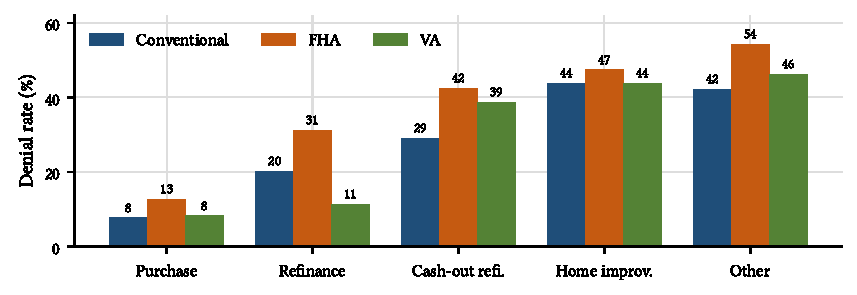
\includegraphics[width=0.82\textwidth]{figures/fig_products.pdf}
\caption{Denial rate by loan purpose and type. FHA is denied more than conventional for every purpose, but the purpose gaps (8\% to over 40\%) are larger than the type gaps. USDA (37,386 decisioned, almost all purchases) is omitted.}\label{fig:products}
\end{figure*}

\subsection{Risk and the Composition of Gaps (SQ2)}

\textbf{Denial and DTI.} Figure~\ref{fig:dti} shows that denial is flat between \drDTImidMin\% and \drDTImidMax\% at every reported DTI value from 30\% to 49\%, then rises to \drDTIfiftySixty\% at 50--60\% and \drDTIoverSixty\% above 60\%. A jump test compares the change between adjacent DTI values with the mean step inside 36--49 (Table~\ref{tab:jump}). For conventional loans denial rises from \drConvFortynine\% at DTI 49 to \drConvFiftySixty\% at 50--60, an excess of \jumpConvMain{} points (95\% CI \jumpConvMainLo--\jumpConvMainHi), while the step from 42 to 43 is \jumpConvFortythree{} points and placebo cuts at 40 and 47 are not significant for conventional loans. Two cautions apply. The 50--60 value is one bin of eleven DTI values, so the main step compares a single value with a bin average and is not a regression discontinuity estimate. And with samples this large even small steps are statistically significant (for FHA, \jumpFHAFortythree{} points at 43 and \jumpFHAFortyfive{} at 45), so the conclusion rests on the size of the step, about 65 points against less than 1, not on significance. Applications bunch at exactly 49 (\bunchConv{} times the mean count at 44--48). FHA and VA show small jumps at 50 (\jumpFHAMain{} and \jumpVAMain{} points).

\emph{Why it matters.} The binding underwriting limit for conventional loans in 2024 is 50\%, consistent with the GSE automated underwriting cap \citep{fanniemae_dti}, not the 43\% limit of the Qualified Mortgage rule that a price-based test replaced \citep{cfpb2020qm}; applicants or loan officers appear to structure applications just under it. \emph{Alternatives.} DTI is reported by the lender after underwriting, so bunching may partly reflect recalculation rather than borrower behavior, and denials above 50\% may route to FHA rather than fail outright, which the heatmap supports: at DTI 50--60 and CLTV 95--100 (\fhaHighDTIcltvHundred\% FHA) denial is only \drHighDTIcltvHundred\% (Figure~\ref{fig:heatmap}, Appendix~\ref{app:supp}).

\begin{figure*}[t]
\centering
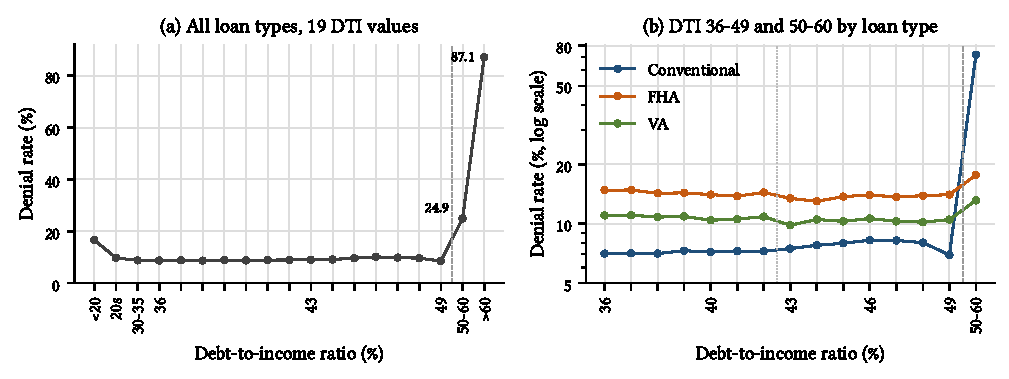
\includegraphics[width=0.96\textwidth]{figures/fig_dti.pdf}
\caption{Denial rate by debt-to-income ratio, usable decisioned applications. (a) All 19 reported values; (b) single values 36--49 and the 50--60 bin by loan type (log scale). Dashed line: the cut between 49 and 50--60; dotted line in (b): the 43\% cut.}\label{fig:dti}
\end{figure*}

\begin{table}[t]
\caption{DTI jump test: change in denial rate between adjacent DTI values minus the mean step within 36--49 (percentage points). $^{*}$ 95\% confidence interval excludes zero. Bunching: applications at DTI 49 divided by the mean at 44--48.}\label{tab:jump}
\footnotesize
\setlength{\tabcolsep}{3.2pt}
\begin{tabular}{lrrrrrr}
\toprule
& Main & \multicolumn{2}{c}{Checks} & \multicolumn{2}{c}{Placebos} & \\
\cmidrule(lr){2-2}\cmidrule(lr){3-4}\cmidrule(lr){5-6}
Scope & 49$\to$50--60 & 42$\to$43 & 44$\to$45 & 39$\to$40 & 46$\to$47 & Bunching \\
\midrule
\tabin{tables/jump.tex}
\bottomrule
\end{tabular}
\end{table}

\textbf{Low DTI is not low risk.} Applications below 20\% DTI are denied at \drDTIlowTwenty\%, against \drDTItwentyThirty\% at 20--30\%. They have higher incomes (median \$\lowDTIincome{}k versus \$\midDTIincome{}k) and lower CLTV, and credit history is cited in \lowDTIcredit\% of their denials against \midDTIcredit\% at 20--30\%. Low DTI therefore marks a different applicant pool, not a safer one: \lowDTInonPurchase\% of these applications are not purchases (against \midDTInonPurchase\% at 20--30\%), their median CLTV is \lowDTIcltv\%, and their denials turn on credit history rather than affordability. The same pattern appears in CLTV: denial is \drCLTVlow\% at CLTV $\le$80\%, where cash-out refinancing concentrates (\convCashoutLeEighty\% of conventional cash-out originations), \drCLTVmid\% at 90--95\%, and \drCLTVhigh\% above 100\%.

\textbf{Decomposition.} Table~\ref{tab:kitagawa} splits each gap by Kitagawa decomposition \citep{kitagawa1955} over the 90 risk cells into composition (different risk mix) and rate (different denial at equal risk), averaging the two groups' weights. The rate part is also shown at each group's own mix, because the share explained by risk depends on that choice. Gaps here are measured on the usable sample and so differ from those of Section~\ref{sec:sqone}, which uses all decisioned applications (\gapFHAdecisioned{} points for FHA versus conventional and \gapCOdecisioned{} for cash-out versus purchase).

\begin{table}[t]
\caption{Kitagawa decomposition of denial gaps over 90 risk cells (percentage points, group A minus group B). Last column: cells where A is denied more than B, out of cells with both groups.}\label{tab:kitagawa}
\footnotesize
\setlength{\tabcolsep}{2.6pt}
\begin{tabular}{lrrrrrr}
\toprule
& & & & \multicolumn{2}{c}{Rate at mix of} & \\
\cmidrule(lr){5-6}
A vs B & Gap & Comp. & Rate & A & B & A higher \\
\midrule
\tabin{tables/kitagawa.tex}
\bottomrule
\end{tabular}
\end{table}

\emph{FHA versus conventional (H1).} With averaged weights, \kgFHAcompShare\% of the \kgFHAgap{}-point gap is composition. That share is not meaningful on its own: the rate gap is \kgFHAatFHA{} points at the FHA mix but \kgFHAatConv{} at the conventional mix, and cell-level gaps run from \kgFHAmin{} to \kgFHAmax{} points (FHA higher in \kgFHAhigher{} cells, lower in \kgFHAlower). FHA approves more in the high-DTI, high-CLTV cells that are its purpose and denies more where conventional borrowers concentrate, consistent with applicants in those cells choosing FHA because of weaker credit, which HMDA does not report. Two cautions: the cells do not condition on loan purpose, and cash-out refinancing is \coShareFHA\% of FHA but \coShareConv\% of conventional decisions, so part of the rate component may reflect purpose; and the extreme cell gaps come from small cells (the smallest holds \minFHAcell{} FHA applications). \emph{Cash-out versus purchase.} The \kgCOgap{}-point gap is almost all rate (\kgCOrate{} points) and cash-out is denied more in \kgCOhigher{} of 90 cells; credit history is cited in \creditCashout\% of cash-out denials against \creditPurchase\% of purchase denials, while DTI is the leading reason for purchases (\dtiReasonPurchase\%). Lenders appear to treat equity extraction as riskier at the same measured ratios.

\textbf{Pricing.} Within conventional loans, cash-out loans pay \psCOconvGap{} points more spread than purchases, all of it within cells (rate part \psCOconvRate{}; purchase coverage \psCOconvCov\%); the gap is unchanged (\psCOconvGapFive) when spreads above 5 points are dropped. For VA the within-cell gap is larger (\psCOvaRate{} points) and composition offsets it (\psCOvaComp). Only \fhaCashoutGtEighty\% of FHA cash-out loans exceed 80\% CLTV, so they share cells with only \psCOfhaCov\% of FHA purchases; we do not interpret that decomposition.

\subsection{Geography (SQ3)}

Risk standardization matters less across states than across products. The standard deviation of state denial rates falls from \sdStateRaw{} to \sdStateStd{} points after standardization, and the between-state variance of $O/E$ net of binomial noise gives $\tau=\tauState$ (\nStates{} jurisdictions: 50 states and DC). Across the \nMSA{} MSAs with at least 1,000 usable applications, $\tau=\tauMSA$ and \msaOutside\% lie outside 95\% funnel limits \citep[Figure~\ref{fig:funnel}b;][]{spiegelhalter2005}. LMI tracts are denied at \drLMI\% against \drNonLMI\% elsewhere; of the \kgLMIgap{}-point gap, \kgLMIrate{} points remain within risk cells (LMI higher in \kgLMIhigher{} of 90 cells), and a within-cell gap of \lmiTypeMin{} to \lmiTypeMax{} points remains inside conventional, FHA, and VA loans separately. LMI originations are also smaller (median \$\loanLMI{} versus \$\loanNonLMI). Puerto Rico ($O/E=\oePR$) and the \nNoState{} usable applications without a state ($O/E=\oeNoState$) are reported separately; \noStateNoTract{} of the 8,643 decisioned ones also lack a tract, so they are not a regional group.

\emph{Alternatives.} The LMI residual is not evidence of different treatment: credit scores, which HMDA omits, may differ between LMI and other tracts, and the risk cells use only three ratios.

\subsection{Lenders (SQ4)}

The \nLenderEightTwelve{} lenders with at least 500 decisioned applications hold \lenderShare\% of decisions; \nLender{} also have at least 80\% usable applications. Their $O/E$ ratios are far more dispersed than those of MSAs (Figure~\ref{fig:funnel}): $\tau=\tauLender$ against \tauMSA, and \lenderOutside\% of lenders lie outside the 95\% limits (\lenderOutsideHigh\% outside 99.8\%). The distribution is skewed: the median lender has $O/E=\lenderMedianOE$, with a long upper tail above 2, and \nZeroDen{} lenders recorded no denials. The expected rate is weighted by applications and therefore dominated by large lenders, so most lenders lie below 1 and the share outside the funnel, which is centred on 1, partly reflects this; $\tau$ measures spread around the mean ratio. Weighted by applications, $\tau$ is \tauLenderW{} for lenders and \tauMSAW{} for MSAs. Median $O/E$ is \agHUD{} for the \nHUD{} lenders supervised through HUD (independent mortgage companies) and \agCFPB{} for large banks supervised by the CFPB.

\begin{figure*}[t]
\centering
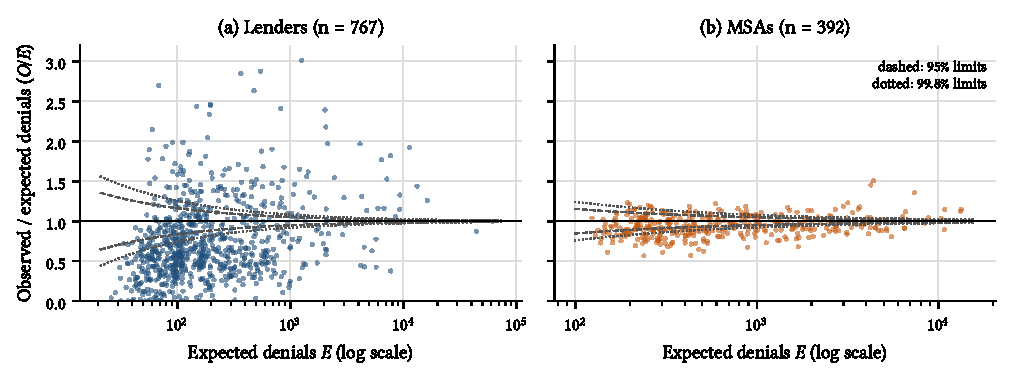
\includegraphics[width=0.96\textwidth]{figures/fig_funnel.pdf}
\caption{Funnel plots of observed to expected denials. Limits use the median ratio of binomial variance to $E$. One lender with $O/E>3.2$ is not drawn.}\label{fig:funnel}
\end{figure*}

Because an MSA ratio pools many lenders, we also fit additive lender and MSA effects on residual denial (denied minus expected), an AKM-type design \citep{akm1999} on the connected set of \twLenders{} lenders, \twMSA{} MSAs, and \twRecords{} applications (median \twMedianMSA{} MSAs per lender). Signal variance is the covariance of effects estimated on two random halves of each lender--MSA cell, which removes noise and limited-mobility bias \citep{andrews2008}. The lender effect has a signal standard deviation of \twLenderSD{} points against \twMSASD{} for MSAs, a ratio of \twRatio{} (about \twVarRatio{} in variance). The correction changes little here (\twLenderFullSD{} points before it), because only \twLeTwoShare\% of lenders operate in two or fewer MSAs. The effects come from 40 fixed alternating iterations; convergence was not monitored. The result is robust: $\tau$ is \tauLenderConv{} within conventional and \tauLenderFHA{} within FHA (rank correlation with the main ratio \rhoConv{} and \rhoFHA), between \tauSensMin{} and \tauSensMax{} across cell, lender-size, and usable-share thresholds, and rankings by raw denial barely change when withdrawn and incomplete applications enter the denominator ($\rho=\rhoDef$). Pricing shows the same order: the spread $\tau$ is \spreadTauLender{} points across \nSpreadLender{} lenders against \spreadTauMSA{} across MSAs. Lender concentration in an MSA (median HHI \hhiMedian, 10th--90th percentile \hhiPten--\hhiPninety) is only weakly related to its denial ratio ($\rho=\rhoHHI$).

\emph{Why it matters.} For a borrower, risk-adjusted denial differs about four times as much across lenders as across metropolitan areas, measured in standard deviations; for a supervisor, lender-level outliers rather than regional ones are where review is informative. \emph{Alternatives.} Lenders attract different credit profiles and differ in how many weak applications they discourage before a formal decision, so lender variance is an upper bound on differences in credit policy.

\section{Pandas Implementation}

The Pandas notebook streams the Parquet file in 200,000-row batches with PyArrow, profiles every field with vectorized string kernels, counts exact duplicates with a 64-bit row hash, and keeps only the 24 raw columns the analysis needs. Features are built with vectorized \fd{np.select} and lookups from the rules file; before grouping, missing keys such as an absent state are converted to the code \fd{NA}, so they form a group as they do in Spark. The two-way model alternates lender and MSA means with \fd{numpy.bincount}, and the prediction step uses scikit-learn. On a Kaggle CPU session (4 cores, 30 GiB) the full notebook runs in \rtPandas{} minutes.

\section{PySpark Implementation}

The PySpark notebook (Spark 4.0.4 in local mode on all four cores, driver memory set to 60\% of the memory available at start; session start \sparkInitMain{} s) reads the same Parquet file and computes the field profile in one aggregation of 693 conditional counts. Cleaning uses \fd{filter}, \fd{withColumn}, and \fd{when}; descriptive and decomposition tables use \fd{groupBy}/\fd{agg}; the Transmittal Sheet and cell rates are attached with broadcast \fd{join}s; window functions rank lenders within agency and split each lender--MSA cell into halves with \fd{row_number} ordered by a fixed hash and the row identifier. The connected set is found by label propagation, and each iteration of the two-way model is cut with \fd{localCheckpoint}, because otherwise the query plan grows with every iteration. Medians use exact \fd{percentile}; \fd{percentile_approx} is computed only to measure its error. Logistic regression is refit in MLlib on the same lender folds. The notebook runs in \rtSpark{} minutes on the same machine.

\section{Correctness Comparison Between Pandas and Spark}

A separate script compares six required outputs, a full field profile, and every key analysis number that both notebooks write. Counts must match exactly; means and rates within a relative tolerance of $10^{-9}$, and the iterative two-way results within $10^{-6}$. Table~\ref{tab:eqvalues} shows representative values from both engines and Table~\ref{tab:eqsummary} the full comparison.

\begin{table}[t]
\caption{Selected quantities computed independently by Pandas and Spark.}\label{tab:eqvalues}
\footnotesize
\setlength{\tabcolsep}{3pt}
\begin{tabularx}{\columnwidth}{Lrrc}
\toprule
Quantity & Pandas & PySpark & Agree \\
\midrule
\tabin{tables/eq_values.tex}
\bottomrule
\end{tabularx}
\end{table}

\begin{table}[t]
\caption{All comparisons. Exact agreement is required for counts; floating-point results within the stated tolerance.}\label{tab:eqsummary}
\footnotesize
\setlength{\tabcolsep}{3pt}
\begin{tabularx}{\columnwidth}{Lrrc}
\toprule
Output & Values & Max.\ rel.\ diff. & Agree \\
\midrule
\tabin{tables/eq_summary.tex}
\bottomrule
\end{tabularx}
\end{table}

All \eqTotal{} values agree; the largest difference, $\eqMaxDiff\times10^{-12}$, comes from the order of floating-point summation in the two-way iteration. Spark's \fd{percentile_approx} differs from the exact median by up to \approxErr\% (relative), so reported medians are exact. Three known sources of disagreement are removed by design rather than by adjustment: missing group keys, which Pandas drops by default and Spark keeps, are coded \fd{NA} in both; window ordering always ends with the row identifier, so ties split the same way; and both engines read strings from Parquet, so \fd{NA} is never turned into a null by a CSV reader. Both notebooks were first run on a synthetic file with the same schema, where the same comparison script reported full agreement before the real run. Agreement shows that the two implementations are consistent, not that the rules are right: both follow the same rules file, and the independent check is the Data Browser comparison of Section~2. The predictions are not expected to match exactly across libraries; MLlib and scikit-learn logistic regressions correlate at \corrMLlib{} out of fold, with identical fold assignments.

\section{Performance and Scalability Experiment}

\textbf{Design.} Following the instructor's guidance, replicated data are used only for this benchmark. The input is a 15-column table of the core sample (\nCore{} rows at 100\%), sampled at 10, 25, and 50\% by a hash of the row identifier and replicated 2, 4, and 8 times with shifted identifiers; because Pandas still fit at 8$\times$, replication continued to 16$\times$. Replication multiplies rows but keeps the number of lenders and counties fixed, so grouping cost may grow less than it would on new data of that size. Workloads: (W0) read the original 4.64 GB CSV with all 99 fields (Pandas loads it into memory; Spark, with column pruning switched off, splits every row into its fields and counts rows without keeping them); (W1) denial rate and mean loan amount by loan type $\times$ purpose; (W2) denial rate for each valid county; (W3) broadcast join with the Transmittal Sheet, lender $O/E$, ranking within agency, and ten iterations of the two-way model. Each engine and size runs in its own process on the same Kaggle machine (4 CPUs, \ramTotal{} GB RAM, Pandas 2.3.3, PySpark 4.0.4). Memory of the process tree, including Spark's JVM, is sampled every 0.2 s, and a run is stopped at \budget{} GB, a budget we set at 90\% of RAM (``OOM'' below means this stop, not an operating-system error). Each measure is the median of five runs after one warm-up. Pandas time is reported \emph{warm} (data already in memory) and \emph{cold}, the sum of the median time to read the whole 15-column table and the median warm time; Spark time is reported without cache (read and compute in one action) and on a cached table, with session start and cache building timed separately. The cold comparison is therefore not symmetric: Pandas reads all 15 columns, while Spark reads only the four or five a query uses. At 100\% the two engines return equal W1 and W2 results and W3 results within $\perfEqThree$.

\begin{table*}[t]
\caption{Median time (s) with data read from Parquet: Pandas cold versus Spark without cache, excluding Spark session start (\initMin--\initMax{} s). Speedup $=T_\text{Pandas}/T_\text{Spark}$. OOM: stopped at the \budget{} GB memory budget.}\label{tab:perf}
\small
\setlength{\tabcolsep}{4pt}
\begin{tabular}{lrrrlrrrlrrr}
\toprule
& & \multicolumn{4}{c}{W1: group by type $\times$ purpose} & \multicolumn{4}{c}{W3: join, $O/E$, window, two-way} & \multicolumn{2}{c}{Peak memory (GB)} \\
\cmidrule(lr){3-6}\cmidrule(lr){7-10}\cmidrule(lr){11-12}
Size & Rows (M) & Pandas & Spark & Faster & Speedup & Pandas & Spark & Faster & Speedup & Pandas & Spark \\
\midrule
\tabin{tables/perf_main.tex}
\bottomrule
\end{tabular}
\end{table*}

\begin{figure*}[t]
\centering
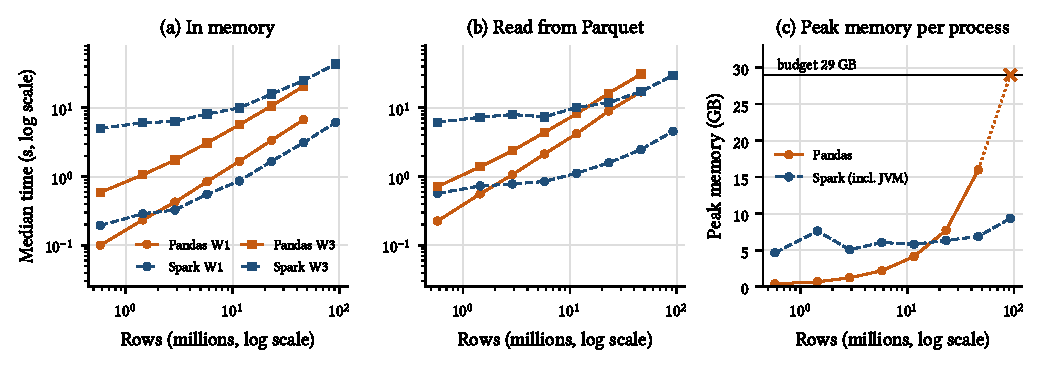
\includegraphics[width=0.96\textwidth]{figures/fig_perf.pdf}
\caption{Scaling of time and memory. (a) Median time of W1 and W3, Pandas cold and Spark without cache. (b) Peak memory of the whole process, including Spark's JVM; the cross marks the run stopped at the budget.}\label{fig:perf}
\end{figure*}

\textbf{Results.} (1) \emph{Which is faster?} It depends on size and workload (Table~\ref{tab:perf}, Figure~\ref{fig:perf}a). For the grouped aggregation W1, Pandas is faster up to 25\% (1.4 million rows); from 50\% Spark is faster, by \spWOneEight{} times at 8$\times$. For the iterative W3, Pandas is faster up to 2$\times$ (11.6 million rows) and Spark from 4$\times$. Reading the full table is \loadShareEight\% of the Pandas cold time for W1 at 8$\times$. With the data already in memory (Table~\ref{tab:perfdetail}), Pandas ties Spark on W1 at 100\% (\warmWOneFull{} against \spWOneFull{} s) and Spark is \warmSpWOneEight{} times faster at 8$\times$; on W3 Pandas stays faster through 4$\times$ (\warmWThreeFour{} against \spWThreeFour{} s) and Spark is \warmSpWThreeEight{} times faster at 8$\times$. The crossover thus lies between the two comparisons, depending on whether the table must be reloaded. (2) \emph{Does the ratio change with volume?} Yes: Pandas time grows linearly with rows, while Spark's has a fixed floor of about 0.6 s for W1 and 6 s for W3 that is amortized as data grow. (3) \emph{Spark overheads.} Session start takes \initMin--\initMax{} s, more than any Pandas run below 2$\times$; each of the ten W3 iterations launches Spark jobs on small tables, a fixed cost consistent with W3 needing more data than W1 before Spark wins. Caching did not pay: building the cache takes \cbFull{} s at 100\% and \cbEight{} s at 8$\times$, and at 4$\times$ and above cached runs of all three workloads were slower than uncached ones (Appendix~\ref{app:supp}, Table~\ref{tab:perfdetail}), consistent with a Parquet read pruning the table to the four or five columns a query needs while the cache holds all 15. (4) \emph{Memory.} Pandas memory grows by about \pdPerMillion{} GB per million rows, from \pdMemFull{} GB at 100\% to \pdMemEight{} GB at 8$\times$; at 16$\times$ (\oomRows{} million rows) it reached the budget during W3 and was stopped, while Spark peaked at \spMemSixteen{} GB; this limit is that of our implementation, which copies the table when it filters the usable rows. Parsing the full CSV exceeded the budget with both the C and PyArrow engines, while Spark parsed it in \wzSparkTime{} s with \wzSparkPeak{} GB. At small sizes Spark uses more memory than Pandas (\spMemTen{} versus \pdMemTen{} GB at 10\%) because the JVM reserves its heap. (5) \emph{When is Spark preferable?} For raw-file parsing and for any table approaching the memory limit, and, on these four cores, for simple aggregations above about 3 to 6 million rows, depending on whether the table is reloaded. For interactive work on the 4.1 million-row usable sample, Pandas is simpler and fast enough.

\section{Optional Predictive Analysis}

\textbf{Target and use.} The target is denial among usable decisioned applications (base rate \baseRate\%). The model is used for one purpose: as an alternative expected value in $O/E$, to test whether lender rankings depend on the coarse risk cells. \textbf{Inputs.} DTI ordinal, CLTV, loan-to-income, loan amount, income, loan type, and purpose: information available at submission. Excluded are post-decision fields (denial reasons, interest rate, costs, purchaser), race, ethnicity, sex, and age, and the lender and location identifiers that the $O/E$ comparison evaluates. \textbf{Leakage.} Missingness depends on the outcome (loan term is missing in \missTermDen\% of denials and \missTermApp\% of approvals; DTI in \missDTIDen\% versus \missDTIApp\%), so the model uses only complete cases without imputation. \textbf{Procedure.} Five folds are assigned by a hash of the lender identifier, so no lender appears in both training and test data, and all metrics are out of fold.

\begin{table}[t]
\caption{Out-of-fold performance on \nUsable{} applications, lender-grouped five-fold split. CITL: calibration in the large (mean predicted minus observed); slope: calibration slope.}\label{tab:pred}
\footnotesize
\setlength{\tabcolsep}{3pt}
\begin{tabular}{lrrrrr}
\toprule
Model & ROC-AUC & PR-AUC & Brier & CITL & Slope \\
\midrule
\tabin{tables/pred.tex}
\bottomrule
\end{tabular}
\end{table}

Gradient boosting ranks better than logistic regression (ROC-AUC \aucGB{} versus \aucLR) and both are well calibrated (slopes near 1; Appendix~\ref{app:supp}, Figure~\ref{fig:calibration}). Replacing the cell-based expectation with either model leaves lender rankings almost unchanged (Spearman $\rho=\rhoPredLR$ and \rhoPredGB), so the lender dispersion in SQ4 is not an artifact of coarse cells. \emph{Limitations.} Without credit scores the model ranks risk only partly, and income and loan size are correlated with protected characteristics; the model is not suitable for decisions about individual applicants.

\section{Financial Interpretation and Limitations}

For \emph{borrowers}, the evidence points to two practical levers: the lender, whose risk-adjusted denial varies about four times as much as the market's in standard deviations, and the DTI threshold at 50\% for conventional loans, above which FHA is the realistic route. For \emph{lenders and analysts}, raw denial comparisons across products mislead: most of the FHA gap is mix, but the remaining difference changes sign across the risk distribution, and cash-out refinancing carries a large denial and price premium at equal measured ratios. For \emph{policymakers}, the former 43\% Qualified Mortgage limit leaves only a \jumpConvFortythree-point step in 2024 conventional denials, while the 50\% GSE cap leaves a \jumpConvMain-point step, and the LMI gap is mostly within risk cells, which calls for data on credit scores before any conclusion about treatment.

\textbf{Limitations.} (i) Credit score, the main omitted variable, differs systematically across products and tracts: FHA borrowers score about 60 points lower than GSE borrowers \citep{urban2026}. Rate components are therefore upper bounds on differences in treatment, and nothing here is evidence of discrimination. (ii) Applications are self-selected and many weak ones are withdrawn before a decision; withdrawn applications lack DTI and cannot be risk-adjusted. (iii) The risk cells use three ratios; the model-based check reduces but does not remove this concern. (iv) The data cover one year and lenders that report to HMDA; partially exempt lenders report no DTI. (v) The sensitivity check that re-adds the \nOpenEndExempt{} records with an exempt open-end flag, planned in the proposal, has not yet been run. (vi) Performance results come from one 4-core machine in local mode; a cluster would change Spark's fixed costs but not the memory limit of Pandas.

\section{Conclusion}

Across 4.1 million risk-measurable applications, observable risk explains most of the FHA--conventional denial gap on average but not its pattern, explains almost none of the cash-out refinance gap, and shows a sharp underwriting threshold at 50\% DTI rather than 43\%. The lender, not the metropolitan area, is the dominant source of variation in risk-adjusted denial and pricing. Two implementations built from one rules file reproduce every number exactly or to $10^{-12}$, and the performance experiment locates the point where Pandas stops working on this machine (\oomRows{} million rows) and where Spark starts to pay off (from about 3 million rows for aggregation and 23 million for iterative work when the table is read each time, and roughly twice those sizes when the data are already in memory).

\bibliographystyle{ACM-Reference-Format}
\bibliography{references}

\appendix

\section{Variables and Coding Rules Verified in the 2024 File}\label{app:rules}

Table~\ref{tab:rules} lists the fields used for each sub-question and every coding rule applied to them.

\begin{table*}[t]
\caption{Variables and coding rules.}\label{tab:rules}
\small
\begin{tabularx}{\textwidth}{>{\raggedright\arraybackslash}p{0.13\textwidth}L}
\toprule
Item & Rule \\
\midrule
Variables & SQ1: \fd{action_taken}, \fd{loan_type}, \fd{loan_purpose}, \fd{lien_status}, \fd{open_end_line_of_credit}, \fd{occupancy_type}, \fd{loan_amount}. SQ2: \fd{debt_to_income_ratio}, \fd{combined_loan_to_value_ratio}, \fd{income}, \fd{denial_reason_1..4}, \fd{rate_spread}. SQ3: \fd{state_code}, \fd{derived_msa_md}, \fd{county_code}, \fd{tract_to_msa_income_percentage}. SQ4: \fd{lei}, \fd{derived_msa_md}; Transmittal Sheet \fd{respondent_name}, \fd{agency_code}. \\
DTI & Values 36--49 stored as bare numbers, others as bins (\texttt{<20\%}, \texttt{20\%-<30\%}, \texttt{30\%-<36\%}, \texttt{50\%-60\%}, \texttt{>60\%}). 19-level ordinal ($<$20 $=1$, 20--30 $=2$, 30--36 $=3$, 36--49 $=4$--17, 50--60 $=18$, $>$60 $=19$), six bands ($<$30, 30--35, 36--42, 43--49, 50--60, $>$60); no midpoint imputed. With 36--49 as one band (75 cells), lender rankings are unchanged ($\rho=\rhoDTIfive$). \\
CLTV, LTI & CLTV bands $\le$80, 80--90, 90--95, 95--100, $>$100\%; values $\le$0 or $>$250\% flagged. Loan-to-income $=\text{loan amount}/(1000\times\text{income})$, tertile cuts 2.36 and 3.40. \\
Cells & 6 $\times$ 5 $\times$ 3 = 90 risk cells, smallest $n=311$. Extended cells add loan type $\times$ purpose: \nExtCells{} cells; \fallbackShare\% of applications fall back to the risk-cell rate ($n<30$); rankings are unchanged when fallback records are dropped ($\rho=\rhoFallback$). \\
$O/E$ and $\tau$ & $O=$ denials, $E=\sum_i p_i$, $V=\sum_i p_i(1-p_i)$; sampling variance of $O/E$ is $V/E^2$; $\tau^2=\operatorname{Var}(O/E)-\overline{V/E^2}$. National $O/E=\nationalOE$ (the gap from 1 comes only from fallback records). \\
Special codes & \fd{NA} (not applicable or not relied on), \fd{Exempt}/\fd{1111} (partially exempt, about 287,000 records per field), \fd{8888}/\fd{9999} (age); kept as categories, never set to zero. Income in thousands; loan amounts on \$10,000 midpoints. \\
Geography & 50 states and DC; Puerto Rico separate; Guam and the Virgin Islands counted only; records without a state reported separately. Tract income ratio 0 treated as missing; LMI $=$ ratio below 80\%. MSA code 99999 (non-metro) excluded from MSA analyses. \\
Thresholds & Lenders: $\ge$500 decisioned and $\ge$80\% usable; MSAs: $\ge$1,000 usable; cells: $\ge$30; all varied in Table~\ref{tab:sens}. \\
\bottomrule
\end{tabularx}
\end{table*}

\section{Supplementary Results}\label{app:supp}

Figures~\ref{fig:heatmap}--\ref{fig:calibration} and Tables~\ref{tab:sens}--\ref{tab:perfdetail} support the main text.

\begin{figure*}[t]
\centering
\begin{minipage}[b]{0.46\textwidth}\centering
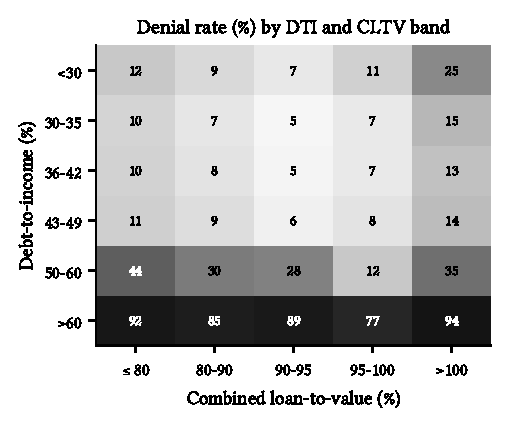
\includegraphics[width=0.86\textwidth]{figures/fig_heatmap.pdf}
\caption{Denial rate (\%) by DTI and CLTV band, usable sample.}\label{fig:heatmap}
\end{minipage}\hfill
\begin{minipage}[b]{0.46\textwidth}\centering
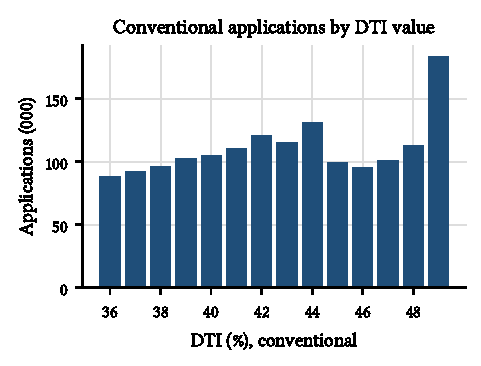
\includegraphics[width=0.86\textwidth]{figures/fig_bunching.pdf}
\caption{Conventional applications by DTI value: bunching at 49.}\label{fig:bunching}
\end{minipage}
\end{figure*}

\begin{figure*}[t]
\centering
\begin{minipage}[b]{0.46\textwidth}\centering
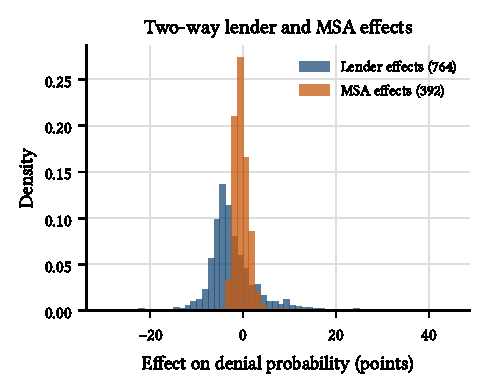
\includegraphics[width=0.86\textwidth]{figures/fig_twoway.pdf}
\caption{Distribution of two-way lender and MSA effects (clipped at $-30$ and $+45$ points).}\label{fig:twoway}
\end{minipage}\hfill
\begin{minipage}[b]{0.46\textwidth}\centering
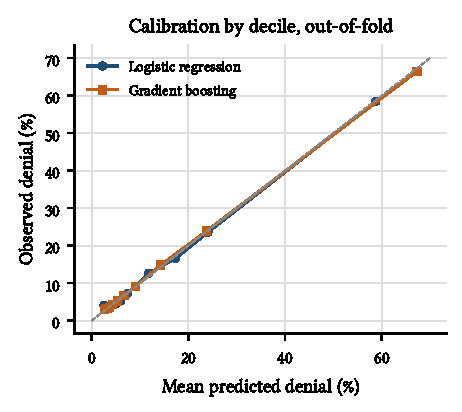
\includegraphics[width=0.86\textwidth]{figures/fig_calibration.pdf}
\caption{Calibration of out-of-fold predictions by decile.}\label{fig:calibration}
\end{minipage}
\end{figure*}

\begin{table*}[t]
\begin{minipage}[t]{0.48\textwidth}
\caption{Sensitivity of lender $O/E$ dispersion to thresholds and scope.}\label{tab:sens}
\footnotesize
\setlength{\tabcolsep}{3pt}
\begin{tabularx}{\textwidth}{Lrrrr}
\toprule
Variant & Lenders & Median $O/E$ & $\tau$ & Out 95\% (\%) \\
\midrule
\tabin{tables/sensitivity.tex}
\bottomrule
\end{tabularx}
\end{minipage}\hfill
\begin{minipage}[t]{0.48\textwidth}
\caption{Field profile excerpt, all \nAll{} records (full profile of 99 fields in the repository).}\label{tab:profile}
\footnotesize
\setlength{\tabcolsep}{3pt}
\begin{tabular}{lrrrr}
\toprule
Field & \fd{NA} & \fd{Exempt} & Numeric & Other codes \\
\midrule
\fd{debt_to_income_ratio} & \dtiNAall & \exemptN & 3,832,520 & binned \\
\fd{rate_spread} & \rsNAall & 287,725 & 5,829,281 & -- \\
\fd{income} & \incomeNAall & 0 & 10,478,765 & 115$^{a}$ \\
\fd{combined_loan_to_value_ratio} & 4,030,609 & 287,538 & 7,941,052 & -- \\
\fd{property_value} & 2,455,474 & 288,601 & 9,515,124 & -- \\
\fd{loan_term} & 204,177 & 286,976 & 11,768,046 & -- \\
\bottomrule
\multicolumn{5}{l}{$^{a}$ Codes \fd{1111}, \fd{8888}, or \fd{9999}.}
\end{tabular}
\end{minipage}
\end{table*}

\begin{table*}[t]
\caption{Performance detail: medians in seconds. Pandas W1--W3 run on data already in memory (warm); Spark ``cached'' runs use a table cached beforehand (build time shown separately), ``direct'' runs read Parquet within the action.}\label{tab:perfdetail}
\small
\setlength{\tabcolsep}{3.6pt}
\begin{tabular}{lrrrrrrrrrrrr}
\toprule
& \multicolumn{4}{c}{Pandas} & \multicolumn{8}{c}{Spark} \\
\cmidrule(lr){2-5}\cmidrule(lr){6-13}
Size & Load & W1 & W2 & W3 & Start & Build cache & W1 cached & W1 direct & W2 cached & W2 direct & W3 cached & W3 direct \\
\midrule
\tabin{tables/perf_detail.tex}
\bottomrule
\end{tabular}
\end{table*}

\section{Reproducibility}\label{app:repro}

Four Kaggle notebooks implement the project: \emph{HMDA v1 pandas}, \emph{HMDA v1 pyspark}, \emph{HMDA v1 performance}, and \emph{HMDA v1 check equivalence} (version 1 of each, run on 6--7 November 2026). Inputs are three private datasets: the converted Parquet file, the configuration (\fd{rules.yaml} 1.1 and \fd{expected.yaml}), and the original FFIEC files imported by URL (LAR CSV and Transmittal Sheet), so no notebook needs Internet access. Each notebook checks its counts against \fd{expected.yaml} and writes every table and key number to \fd{results/}; the tables, figures, and run-dependent numbers in this report are written from those files by a script rather than typed by hand.

\end{document}
